\chapter{Requirement Analysis}
\label{chapter:requirement-analysis}

In the waterfall model, as proposed by Royce, requirements analysis is typically the first phase of the development process \cite{royce70}. This phase involves gathering, documenting, and analyzing the needs and expectations of stakeholders to define the scope and objectives of the software project \cite{Hausen}. The objective of requirements analysis is to pinpoint the user needs and translate them into explicit, quantifiable, and attainable requirements that the software development team can employ to design and build the system \cite{Walker_2023}.

According to Walker \cite{Walker_2023}, within a large organization, this phase is usually carried out by diverse team. Business Analysts identify and document system needs, while Project Managers oversee the process. Developers use these requirements to design the system, and Testers validate them. Stakeholders provide essential input, and Subject Matter Experts offer specialized knowledge to help ensure the requirements are accurate and complete.

According to Geogy and Dharani \cite{Geogy2016}, one of the major challange in this phase is determining what needs to be constructed, as unlike other phases in development, errors in this phase can have far-reaching consequences if identified later on. They also stated that, one of the primary hurdles in the requirements specification process is striking a balance between providing sufficient detail for clear understanding without overly constraining the system.

Hence, to properly define the project requirements, the following steps are taken \cite{Simplilearn_2023}:

\subsubsection{Identify Key Stakeholders and End-Users}
In the initial phase, it is imperative to identify key stakeholders who hold significant influence over the project, playing a crucial role in determining the project's scope. Additionally, pinpointing the end-users, as the primary beneficiaries of the product, is equally imperative. For this project, the end-users will be the police officers and the administrators of the police department.

\subsubsection{Capture Requirements}
The subsequent step involves gathering requirements from stakeholders and end-users. Various techniques such as one-on-one interviews, focus groups, use cases, and prototypes are employed to capture their specific needs. Each technique serves a unique purpose, from gathering detailed individual requirements to visualizing the product's functionality.

\subsubsection{Categories Requirements}
Once requirements are gathered, they are categorized into functional and non-function requirements. This categorization ensures clarity and avoids potential confusion.

% elaborate requirements categories

\subsubsection{Interpret and Record Requirements}
Following categorization, a meticulous process of interpretation and recording ensues. This involves assessing the feasibility, prioritizing requirements, conducting impact analyses, resolving conflicts, and ensuring precise and detailed descriptions aligned with business objectives.

After a thorough analysis, a comprehensive document detailing the requirements is created and distributed among key stakeholders, end-users, and development teams.

\subsubsection{Sign off}
Finally, to maintain project scope integrity, obtaining a signed agreement from key stakeholders is essential. This signifies a final decision on the requirements and prevents any uncontrolled expansion of the project's scope.

\section{Project Requirements}
\label{section:project-requirements}
Figure \ref{fig:project-requirements-1} and \ref{fig:project-requirements-2} shows the result of the requirement analysis process.

\begin{figure}[!ht]
    \centering
    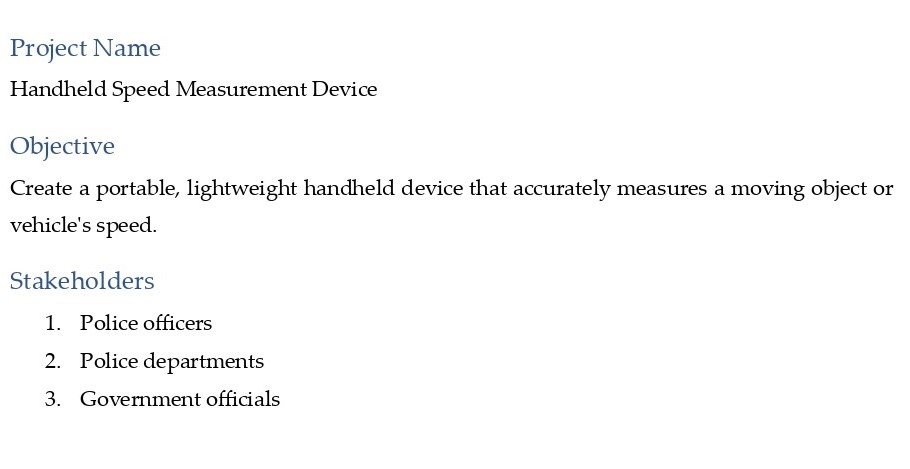
\includegraphics[width=0.9\textwidth]{texs/Part2/chapter2/image/req1.jpg}
    \caption{Project Requirements (1/2)}
    \label{fig:project-requirements-1}
\end{figure}

\begin{figure}[!ht]
    \centering
    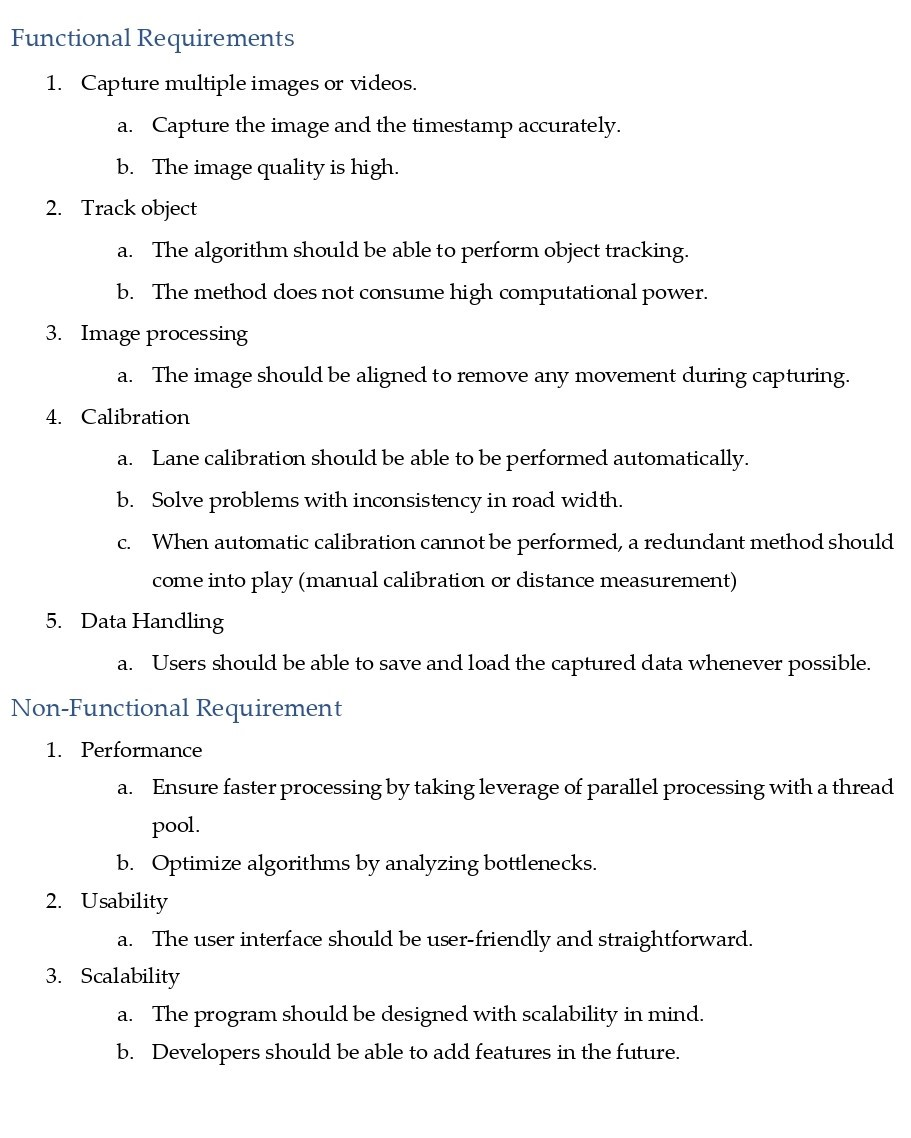
\includegraphics[width=0.9\textwidth]{texs/Part2/chapter2/image/req2.jpg}
    \caption{Project Requirements (2/2)}
    \label{fig:project-requirements-2}
\end{figure}











